\subsection{Trust-Related Behaviors} \label{sec:trbs}
Something that is well accepted among researchers of all disciplines is that trust results in some kind of behavior or action, this idea was highlighted by \citet{Lewis1985-pr}.  \citet{McKnight2001-fa} calls it `trust-related behaviors` (TRBs), which is the term that will be used in this survey.

In the case of a human-AIA relationship these TRBs could include the kinds of tasks the human user assigns to the AIA, or whether the decision a human makes to use a plan produced by the AIA or not. 

\subsubsection{Calibration of Trust-Related Behaviors}
    As yet, trust is not a quantity that can be directly measured. Rather, its relative magnitude must be observed through changes in TRBs, or qualitative surveys -- of the two TRBs are the more objective measure. \citet{Parasuraman1997-co} were interested in understanding the use of automation which they defined as ``\ldots the execution by a machine agent (usually a computer) of a function that was previously carried out by a human''. Within this scope they define the following terms:
    
    \begin{description}
        \item [Misuse:] The overreliance on automation
        \item [Disuse:] The underutilization of automation
        \item [Abuse:] \textbf{I don't think I want to put this in the paper, it is really out of scope\ldots well, it may not be I guess\ldots the AIA could give assurances to help deploy it in the appropriate circumstance} Inappropriate application of automation (where \emph{application} in this case means the choice to deploy automation in a certain context, such as the choice to install a robot in a factory).
    \end{description}

    Here it is proposed that, by extension, the definitions of \emph{misuse}, \emph{disuse}, and \emph{abuse} can apply to the relationship between humans and AIAs. According to the diagram in Figure \ref{fig:SimpleTrust_one_way} the AIA will try to influence the user's TRBs by way of assurances. The goal of an AIA shoud be that the user should not misuse, disuse, or abuse the AIA.
    
    To be more formal, let the total set of TRBs as $\mathcal{T}$. Then as subsets of $\mathcal{T}$ define the set of misue actions as $\mathcal{M}$, the set of disuse actions as $\mathcal{D}$, and the set of abuse actions as $\mathcal{A}$. Next, define the total set of innapropriate TRBs $\mathcal{I}$ as the union of $\mathcal{I} = \mathcal{M}\cup \mathcal{D}\cup\mathcal{A}$. Having defined the set of inappropriate actions, the set of appropriate TRBs can be defined as $\mathcal{U}$, the compliment of the set of inappropriate TRBs $\mathcal{U} = \mathcal{I}^\prime$. This is illustrated in Figure \ref{fig:appropriate_use}, where the set of appropriate actions $\mathcal{U}$ is the gray colored area (i.e. all TRBs \emph{not} in either of the three sets of inappropriate TRBs). \textbf{This is probably too complicated, I could probably just say that $\mathcal{U}$ is the set of all actions not included in either of M,A, or D}.
    
	\begin{figure}[htbp]
    	\centering
     	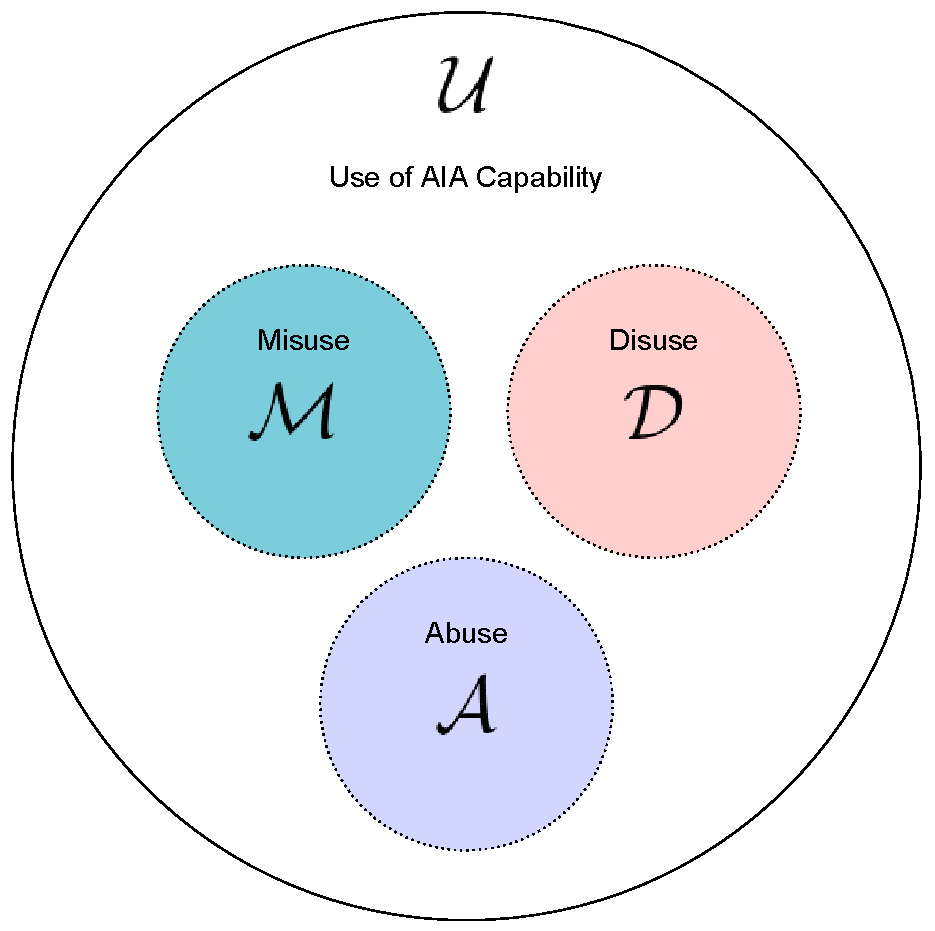
\includegraphics[width=0.4\textwidth]{Figures/misuse_disuse_abuse}
    	\caption{Graphic representing the total space of user actions, in which the inappropriate uses $\mathcal{M}$, $\mathcal{D}$, and $\mathcal{A}$ lie. The set of inappropriate uses $\mathcal{I}$ is the union of $\mathcal{M}$, $\mathcal{D}$, and $\mathcal{A}$. The appropriate set of actions $\mathcal{U}$ is the compliment of $\mathcal{I}$, or the part of $\mathcal{T}$ that does not include $\mathcal{I}$.}
        \label{fig:appropriate_use}
    \end{figure}
    
    Given this definition, in order to ensure that humans use AIAs appropriately, it is critical that the user TRBs be calibrated to elicit behaviors that are within $\mathcal{U}$. This can be done by influencing the user trust. This is a point that, to some extent, has been informally mentioned in \citet{Muir1994-ow,Muir1987-mk,Lillard2016-yg,Lee2004-pv,Hutchins2015-if}. An aim of this paper is to more formally investigate that topic.

    A critical oversight of the those who mention is that they suggest calibrating \emph{trust} as opposed to TRBs. \citet{Dzindolet2003-ts} studied the effect of performance feedback on user's self-reported trust, and found that it increased, however the appropriate TRBs toward the system didn't reflect the level of self-reported trust. This shows the danger of calibrating ``trust'', as opposed to calibrating the TRBs.

    Calibrating TRBs focuses on concrete and measurable behaviors that are universally applicable. In contrast, calibrating trust involves influencing a quantify that is directly immeasurable, and that, when measured indirectly, is subject to the biases, uncertainties, and fundamental differences of humans. Viewing the task from this point of view, the findings of \citeauthor{Dzindolet2003-ts} are not surprising.

    \textbf{I'd like to go off on a little rant about this, but I'm not sure if it is appropriate. There is a TON of literature that talks about calibrating trust. Calibrating trust is asking for trouble, when we actually care about TRBs. VERY LITTLE RESEARCH  (none?) HAS BEEN DONE CONSIDERING ONLY TRBS, IT IS MOSTLY JUST SELF-REPORTED TRUST, WHICH DZINDOLET HAS SHOWN TO BE SHAKY GROUND}

    From the perspective of a benevolent AIA, the user's TRBs should lay within $\mathcal{U}$, this in contrast to a malicious AIA that tries to manipulate the TRBs of a human to overlap $\mathcal{I}$ to some extent. There is a valid argument that many of today's systems that ignore TRBs and assurances are unwittingly malicious in that they do not actively attempt to guide user's TRBs to lay withing $\mathcal{U}$.

    % Generally trust between a human and AI could be depicted as in Figure \ref{fig:SimpleTrust_two_way}, where each has TRBs that must be calibrated, and each provides certain feedback, which will be called assurances, in order to do so. In a more simple scenario, where the AI implicitly trusts the human user the trust relationship can be depicted as shown in Figure \ref{fig:SimpleTrust_one_way}, where only the user has TRBs that are being calibrated.

	% \begin{figure*}[htbp]
        % \centering
        % \begin{subfigure}[t]{0.48\textwidth}
            % \centering
            % 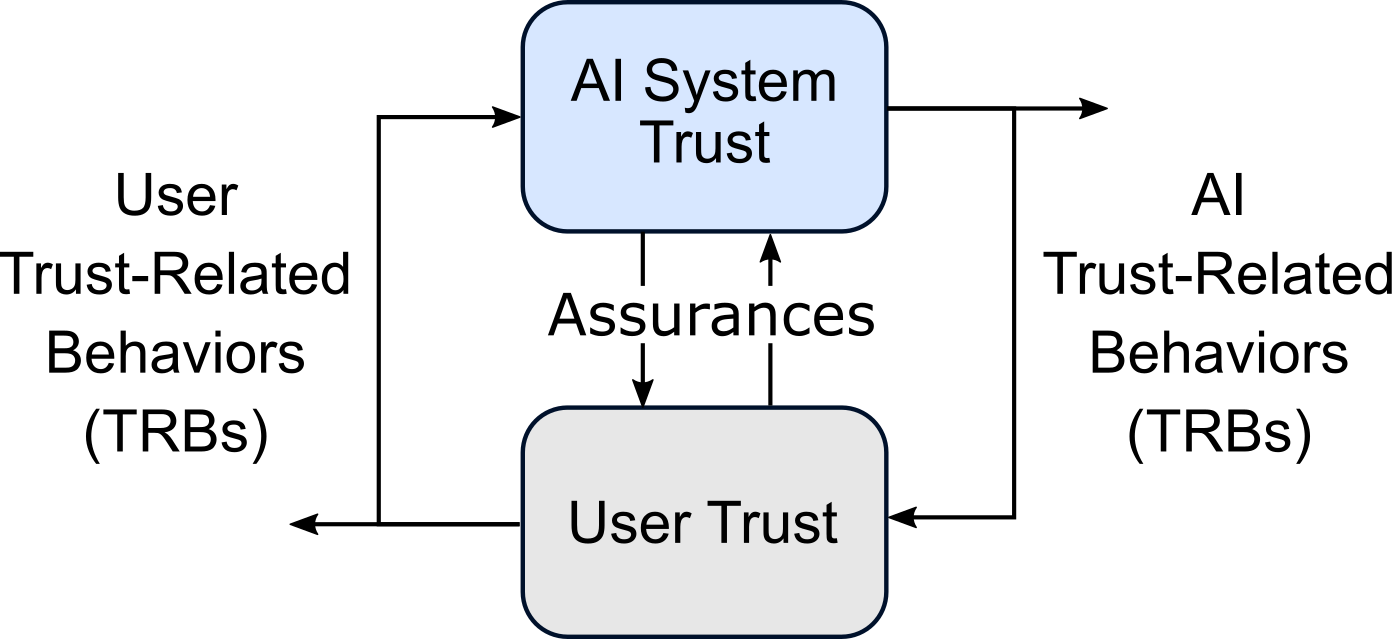
\includegraphics[width=0.95\textwidth]{Figures/SimpleTrust_two_way}
            % \caption{Diagram showing a general case of a two-way trust relationship between an AI and a human. Arrows that are not connected to boxes represent some action outside of the trust loop.}
            % \label{fig:SimpleTrust_two_way}%
        % \end{subfigure}
        % \hfill
        % \begin{subfigure}[t]{0.48\textwidth}
            % \centering
            % 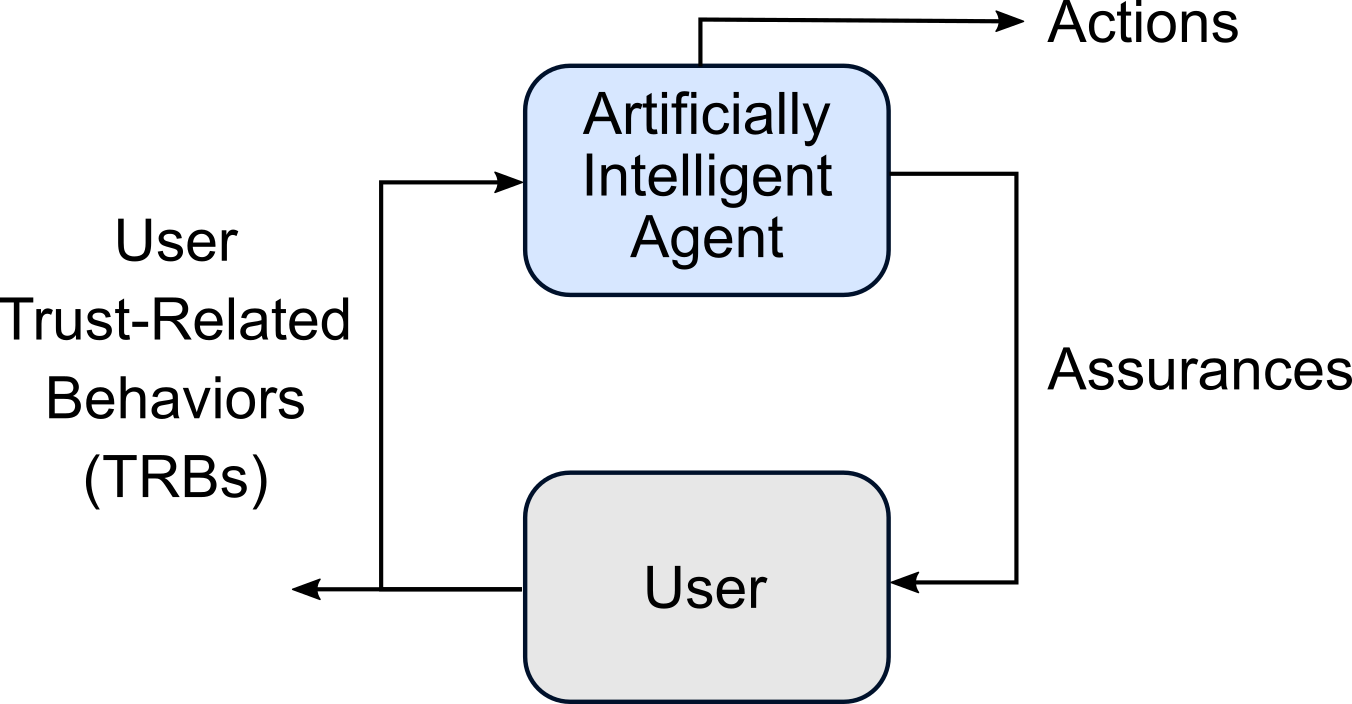
\includegraphics[width=0.95\textwidth]{Figures/SimpleTrust_one_way}
            % \caption{Diagram illustrating a general one-way trust relationship between a human and an AI. In this case the AI has, what could be considered perfect trust in the user.}
            % \label{fig:SimpleTrust_one_way}%
        % \end{subfigure}
        % \caption{Feedback Loops For One and Two-way human-AI Trust Relationships}
        % \label{fig:SimpleTrust}
    % \end{figure}
    
    % Figure \ref{fig:SimpleTrust_dist} serves as a simple example illustrating the possible disparity between the user TRB distribution and the appropriate TRB distribution. In this case assurances would be used to minimize the difference between the two distributions.

	% \begin{figure}[htbp]
        % \centering
         % 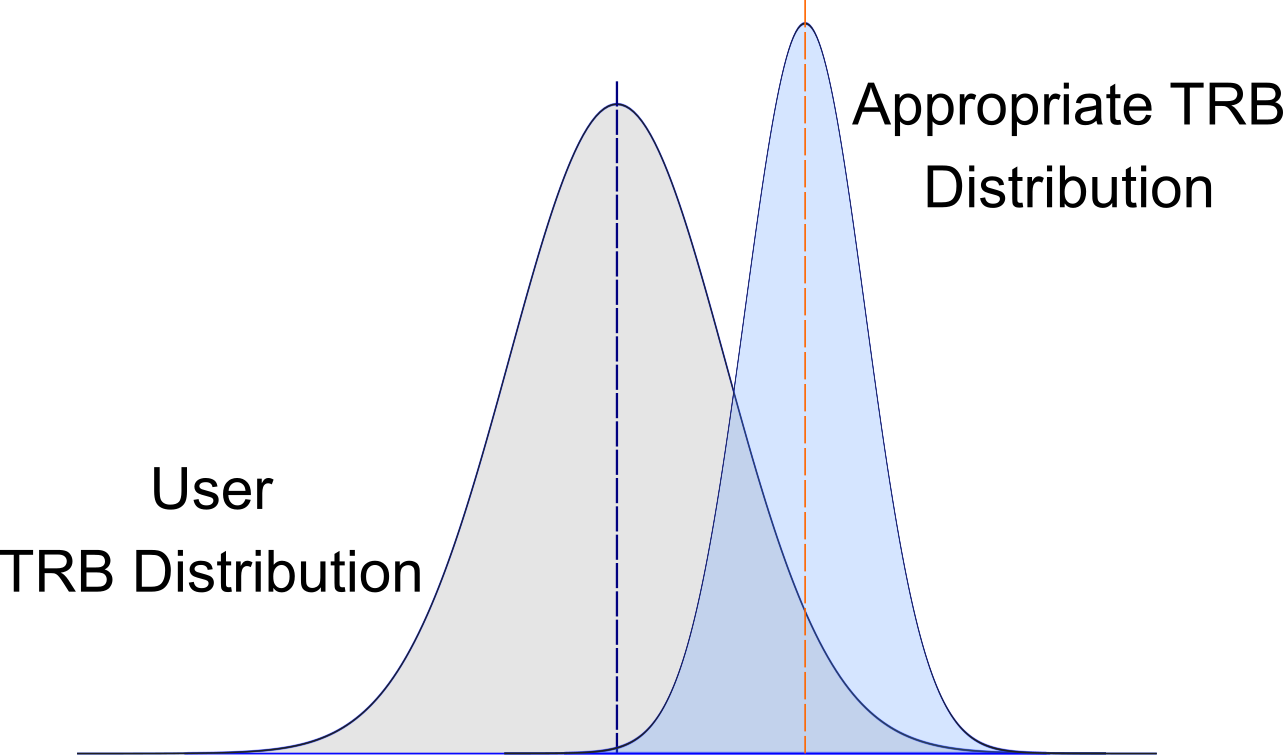
\includegraphics[width=0.4\textwidth]{Figures/SimpleTrust_dist.png}
        % \caption{Diagram illustrating the point that a hypothetical user TRB distribution might not match the appropriate TRB distribution. In this case the AI should provide assurances in order to minimize the difference between the two.}
        % \label{fig:SimpleTrust_dist}
    % \end{figure}
%
